% TikZ figure: Belief simplex partition for a three-state POMDP
% Each region corresponds to the belief points where one alpha vector dominates

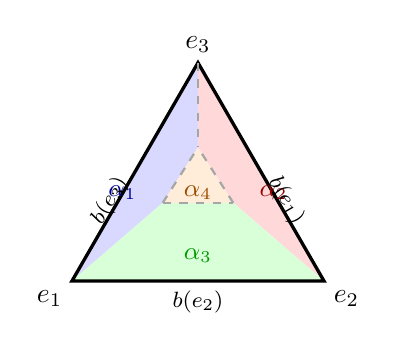
\begin{tikzpicture}[scale=3.2]

  % Define the three vertices of the simplex
  \coordinate (v0) at (0,   0);      % b = (1,0,0): all mass on s0
  \coordinate (v1) at (1,   0);      % b = (0,1,0): all mass on s1
  \coordinate (v2) at (0.5, 0.866);  % b = (0,0,1): all mass on s2

  % Partition boundaries (approximate dividing lines inside simplex)
  \coordinate (c1) at (0.36, 0.31);
  \coordinate (c2) at (0.64, 0.31);
  \coordinate (c3) at (0.50, 0.53);

  % Fill the three regions with light colors
  \fill[blue!15]   (v0) -- (c1) -- (c3) -- (v2) -- cycle;
  \fill[red!15]    (v1) -- (c2) -- (c3) -- (v2) -- cycle;
  \fill[green!15]  (v0) -- (c1) -- (c2) -- (v1) -- cycle;
  \fill[orange!15] (c1) -- (c2) -- (c3) -- cycle;

  % Draw the simplex outline
  \draw[very thick] (v0) -- (v1) -- (v2) -- cycle;

  % Draw partition boundaries
  \draw[thick, dashed, gray!70] (v2) -- (c3);
  \draw[thick, dashed, gray!70] (c1) -- (c3);
  \draw[thick, dashed, gray!70] (c2) -- (c3);
  \draw[thick, dashed, gray!70] (c1) -- (c2);

  % Label vertices
  \node[below left]  at (v0) {$e_1$};
  \node[below right] at (v1) {$e_2$};
  \node[above]       at (v2) {$e_3$};

  % Region labels
  \node[blue!60!black,   font=\small] at (0.20, 0.35) {$\alpha_1$};
  \node[red!60!black,    font=\small] at (0.80, 0.35) {$\alpha_2$};
  \node[green!60!black,  font=\small] at (0.50, 0.10) {$\alpha_3$};
  \node[orange!60!black, font=\small] at (0.50, 0.35) {$\alpha_4$};

  % Axis labels along edges (matching vertex notation e_1, e_2, e_3)
  \node[below, font=\footnotesize] at (0.5, 0) {$b(e_2)$};
  \node[left,  font=\footnotesize, rotate=60] at (0.22, 0.44) {$b(e_3)$};
  \node[right, font=\footnotesize, rotate=-60] at (0.78, 0.44) {$b(e_1)$};

\end{tikzpicture}
